\documentclass[12pt]{article}
\usepackage{amsmath}
\usepackage[rm,tiny,explicit]{titlesec}
\usepackage[margin=1in]{geometry}
\usepackage{subfigure}
\usepackage[subfigure]{tocloft}
\usepackage{etoolbox}
\usepackage{graphicx}
\usepackage{chngcntr}
\usepackage{afterpage}
\usepackage{pdfpages}
\usepackage{fancyvrb}
\usepackage{listings}
\usepackage[euler]{textgreek}
\counterwithin{figure}{section}
\counterwithin{table}{section}
\usepackage[labelfont=bf]{caption}
\usepackage{enumitem}
\setlist{nolistsep}
\usepackage{wasysym}
\usepackage{multirow}
\usepackage{booktabs}
\usepackage[titletoc,toc,title]{appendix}

\renewcommand\cftsecfont{\normalfont}
\renewcommand\cftsecpagefont{\normalfont}
\renewcommand{\cftsecleader}{\cftdotfill{\cftdotsep}}

%Add table padding
\renewcommand{\arraystretch}{1.25} % Default value: 1

\titleformat{\section}{\normalfont\centering\bfseries}{\thesection}{1em}{\MakeUppercase{#1}}
\titleformat{\subsection}{\normalfont\flushleft\bfseries}{\thesubsection}{1em}{#1}
\titleformat{\subsubsection}{\normalfont\flushleft\bfseries}{\thesubsubsection}{1em}{#1}


\setcounter{secnumdepth}{3}
\setcounter{tocdepth}{2}

\renewcommand{\floatpagefraction}{.8}
\renewcommand{\topfraction}{.8}
\renewcommand{\textfraction}{.2}

% required by \up and \down
\usepackage{amsmath}

% add superscripts OUTSIDE of math mode
\newcommand{\up}[1]{$^\text{#1}$}

% add subscripts OUTSIDE of math mode
\newcommand{\down}[1]{$_\text{#1}$}

% remove border from cell
\newcommand{\nob}[1]{\multicolumn{1}{c}{#1}}

% Duct tape Appendix
\newcommand{\app}[2][\null]{
	\clearpage
 	\newpage
 	{
 	 	\centering
 	 	\addcontentsline{toc}{section}{Appendix #2}
% 	 	\textbf{APPENDIX A} \\ \bigskip
		\section*{APPENDIX #2}
 	 	\textbf{#1} \\ \bigskip
 		}
}

\begin{document}  	
	\section{The Team}
		\vfill
		\begin{tabular}{l l}
			Team Name:    & Sensor Network    \\
			\\
			Team Members: & Nick Morley       \\
			              & Jonathan Richards \\
%			              & Daniel Kline\\
			              \\
			Technical Advisor: & Dr. Hovannes Kulhandjian\\
			\\
			Course Instructor: & Dr. Reza Raeisi\\
		\end{tabular}
		\vfill
		\tableofcontents
		\vfill
		\newpage
		 
	\section{Goal}
		\begin{itemize}
			\item Create a system to collect, transport, analyze, store, and visualize sensor data
			\item Control external systems manually or automatically according to sensor inputs
			\item Access user interface anywhere with an internet connection
		\end{itemize}
		
	\section{Objectives}
		\begin{itemize}
			\item Build sensor modules built around existing sensors that interface and draw power from the wireless node
			\item Build wireless nodes that connect to the sensor module over a unified hardware interface. The nodes will form a mesh network to establish communication with the base station
			\item The base station will interface with the nodes and sensors, both reading sensor values and controlling modules. It will also host the database to store historic data and a server to interface with mobile apps
			\item The mobile app will allow the user to interface with our system; reading sensors, configuring nodes, and controlling nodes.
		\end{itemize}
	
	\section{Background}
		\begin{itemize}
			\item Microcontroller Programming and Interfacing
			\item Wireless Communication and Networking
			\item Data Storage, Processing, and Serving
			\item Mobile App Development
		\end{itemize}
 
	 \section{Feasibility}
		 \begin{itemize}
		 	\item ESP8266 Microcontroller
			 	\begin{itemize}
			 		\item Economical (\$15 Development Kit)
			 		\item Integrated WiFi with 400+ m range
			 		\item Interface with multiple sensors
			 	\end{itemize}
		 	\item WiFi Communication
			 	\begin{itemize}
			 		\item Commonly available
			 		\item Use mobile app to configure nodes via WiFi
			 		\item Connect to existing network to access internet
			 		\item Connect mobile device to local network to interface with sensors
			 	\end{itemize}
		 	\item Data Storage, Processing, \& Serving
			 	\begin{itemize}
			 		\item Use Raspberry Pi or router running Linux
			 		\item Store sensor data on USB Drive using SQL server
			 		\item Perform analytics on data
			 		\begin{itemize}
				 		\item Energy Usage
				 		\item Run time
				 		\item Temperature Variations
				 	\end{itemize}
			 		\item Configure controllers
			 		\item Send data to mobile device for viewing via websockets
			 	\end{itemize}
			 \item Mobile App Development
				 \begin{itemize}
				 	\item Do initial setup of sensor
				 	\item View sensor data
				 	\item Configure controllers
				 	\item Connect locally or over the internet through online account
				 \end{itemize}
		 \end{itemize}
		 
	 \section{Inputs/Outputs}
		 The logical datapath for the project is diagramed in Figure~\ref{fig:BlockDiagram}. The network diagram for connecting different physical modules are presented in Figure~\ref{fig:NetworkDiagram}. The inputs/outputs are summarized below.
		 \begin{itemize}
		 	\item Sensor Data
		 	\begin{itemize}
		 		\item Temperature
		 		\item Humidity
		 		\item Wind Speed
		 		\item Rainfall
		 		\item Barametric Pressure
		 		\item Voltage / Current
		 		\item Brightness
		 		\item Sound
		 	\end{itemize}
		 	\item Control Data
		 	\begin{itemize}
		 		\item AC / Heater
		 		\item LEDs
		 		\item Outlet
		 		\item Light
		 	\end{itemize}
		 	\item Node Configuration
		 	\begin{itemize}
		 		\item Sampling Rate
		 		\item Precision
		 		\item Control Conditions
		 		\item Network
		 		\item Link to Account		 		
		 	\end{itemize}
		 	\item Plotted Sensor Data
		 	\begin{itemize}
		 		\item Organize sensor data graphically for user
		 	\end{itemize}
		 	\item Sensor Data Analytics
		 	\begin{itemize}
		 		\item Averages
		 		\item Cummulative Totals
		 	\end{itemize}
		 	\item Network Status
		 	\begin{itemize}
		 		\item Nodes online
		 		\item Last sensor readings
		 	\end{itemize}
		 \end{itemize}
	 
		\begin{figure}[h!]
			\centering
			\includegraphics[height=0.8\textwidth, angle=90]{BlockDiagram}
			\caption{The Logical Datapath}
			\label{fig:BlockDiagram}
		\end{figure}
		
		\clearpage
		
		\begin{figure}[h!]
			\centering
			\includegraphics[height=\textwidth, angle=90]{NetworkDiagram}
			\caption{The Physcical Datapath}
			\label{fig:NetworkDiagram}
		\end{figure}
		
		\clearpage
		 
	\section{Project Timeline}
	
		\begin{figure}[h!]
			\centering
			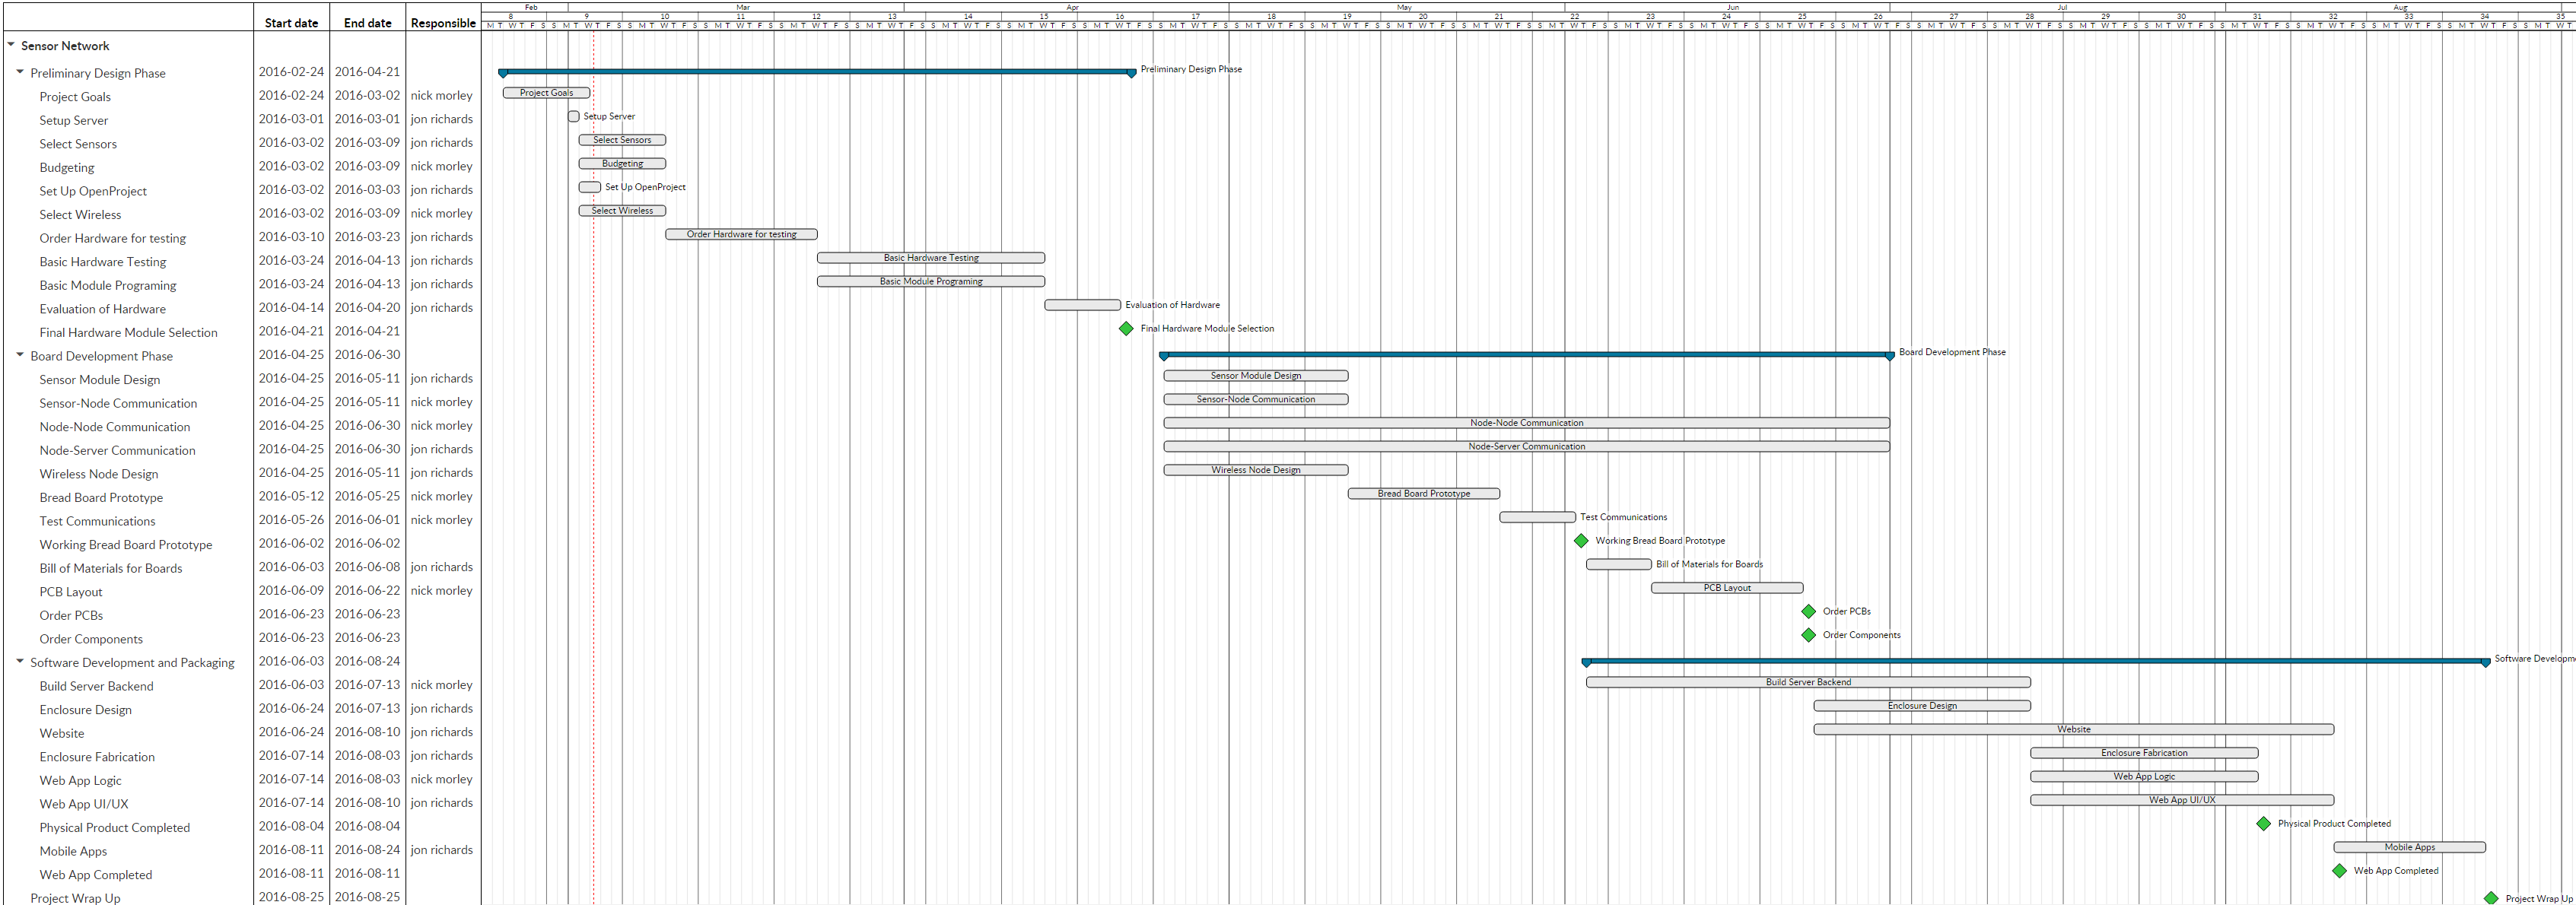
\includegraphics[width=0.85\textheight, angle=90]{GantChart}
			\caption{Gant Chart for Project Timeline}
			\label{fig:NetworkDiagram}
		\end{figure}
		 
		 
%	 \newpage
%	 \section{Approval}
%		\begin{flushleft}
%			I agree to build the above project throughout ECE 186A and 186B.\\
%			\vspace{2em}
%			\begin{tabular}{l l l}
%				\line(1,0){250} & \hfill & \line(1,0){100}\\
%				\textit{Team Member Signature} & & \textit{Date}				
%			\end{tabular}
%			\vspace{2em}\\
%			\begin{tabular}{l l l}
%				\line(1,0){250} & \hfill & \line(1,0){100}\\
%				\textit{Team Member Signature} & & \textit{Date}
%			\end{tabular}
%%			\vspace{2em}\\
%%			\begin{tabular}{l l l}
%%				\line(1,0){250} & \hfill & \line(1,0){100}\\
%%				\textit{Team Member Signature} & & \textit{Date}
%%			\end{tabular}
%			\vspace{5em}
%			
%			I agree to be the formal, technical adivsor to this project.\\
%			\vspace{2em}
%			\begin{tabular}{l l l}
%				\line(1,0){250} & \hfill & \line(1,0){100}\\
%				\textit{Technical Advisor Signature} & & \textit{Date}
%			\end{tabular}
%			\vspace{5em}
%			
%			I approve this project to be a viable capstone project.\\
%			\vspace{2em}
%			\begin{tabular}{l l l}
%				\line(1,0){250} & \hfill & \line(1,0){100}\\
%				\textit{Course Instructor Signature} & & \textit{Date}
%			\end{tabular}
%		\end{flushleft}		 
		 
\end{document}